\section{Deterministic Toy Domain}
\label{sec:appendix_toy}


\begin{figure}%
	\centering
	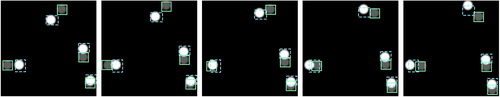
\includegraphics[width=0.99\textwidth]{figures/MOHART/sot_protons.png}
% 	\vspace{-3mm}
	\caption{
		\textsc{hart} single object tracking applied four times in parallel and trained to predict the location of each circle three time steps into the future. Dashed lines indicate spatial attention, solid lines are predicted bounding boxes, faded circles show ground truth location at $T+3$. Each circle exerts repulsive forces on each other, where the force scales with $1/r$, $r$ being their distance.
	}
	\label{fig:toy1}
\end{figure} 
%    	\textsc{hart} single object tracking applied four times in parallel. Dashed lines indicate spatial attention, solid lines are predicted bounding boxes at time step $T+3$, faded circles show the ground truth location at $T+3$. A repulsive force acts between each object pair which scales with distance as $1/r$. There is no information exchange between the trackers and each tracker evidently only `attends' to its own object. The fact that the future location is predicted accurately (i.e., much better than linear extrapolation) indicates that \textsc{hart} is able to capture complex motion patterns essentially allowing to draw conclusions about the force field. Shown are consecutive time steps from left to right.

In our first experiment in the toy domain (\Cref{fig:toy1}), four circles each exert repulsive forces on each other, where the force scales with $1/r$, $r$ being their distance. \textsc{hart} is applied four times in parallel and is trained to predict the location of each circle three time steps into the future. The different forces from different objects lead to a non-trivial force field at each time step. Predicting the future location just using the previous motion of one object (\Cref{fig:toy1} shows that each spatial attention box covers only the current object) accurately is therefore challenging. Surprisingly, the single object tracker solves this task with an average of $95\%$ IoU over sequences of 15 time steps. This shows the efficacy of end-to-end tracking to capture complex motion patterns and use them to predict future locations. This, of course, could also be used to generate robust bounding boxes for a tracking task.